\chapter[Steady state full-core MSBR criticality simulation]{Steady state full-core MSBR criticality simulation}

\section{Serpent 2 code overview}

SERPENT is a continuous-energy Monte Carlo neutronics code capable of solving the neutron transport problem by tracking individual neutrons within the problem geometry and using stochastic method to determine chain of events for each neutron \cite{leppanen_serpent_2015}. SERPENT has been under active development at the VTT Technical Research Centre of Finland from 2004, where it was initially conceived as a tool to simplify group constant generation in a high-fidelity Monte Carlo environment. During this period, SERPENT has seen as widely used transport code and number of users grows steadly. Now SERPENT used by more than 500 registered individuals in 155 organisations located in 37 countries around the world. This success is not only a result of the simple and naive cross section generation procedures, but also its high-performance parallelization and user-friendly usage. The burnup calculation capability in SERPENT was established early on, and is fully based on built-in calculation routines, without using any external solvers. A restart features allows performing fuel shuffling or applying any modifications in the input by dividing the calculation into several parts which is crucial for online reprocessing simulations.

Latest version, SERPENT 2, supports advanced geometry types and has advanced burnup capabilities, including online refueling capabilities which are necessarily for neutronic computations of pebble-bed reactors and liquid-fueled \glspl{MSR} \cite{aufiero_extended_2013}. Furthermore, recently was demonstrated multi-physics simulations using SERPENT 2, i.e. coupled calculations with thermal hydraulics, \gls{CFD} and fuel performance codes \cite{leppanen_numerical_2015}. Two-way coupling to thermal hydraulics, CFD and fuel performance codes has been a major topic in Serpent development for the past several years and operate on two levels: 	internal coupling to built-in solvers for fuel behavior and thermal hydraulics and external coupling via a universal multi-physics interface. 

SERPENT 2 can be effectively run in parallel on computer clusters and multi-core workstations. Parallelization at core level is handled by thread-based OpenMP, which has the advantage that all processsors use shared memory space. Calculations can be divided into several nodes by distributed-memory MPI parallelization. SERPENT 2 leverages hybrid OpenMP + MPI parallelized memory management, which allows to achieve significant speed-up in depletion calculations on computer clusters with more than 4'000 cores \cite{leppanen_serpent_2015-1}. In addition to the particle transport simulation, parallelization in the burnup calculation mode divides also the preprocessing and depletion routines between several cores.

All calculations presented in this thesis were performed using SERPENT 2 version 
2.1.28 on Blue Waters’ XK7 nodes. For cross section generation, JEFF-3.2 was employed \cite{oecd/nea_data_bank_jeff-3.2_2014}.

\section{Molten Salt Breeder Reactor description}

The \gls{MSBR} vessel has diameter of 680 cm and a height of 610 cm. It 
contains a molten fluoride fuel-salt mixture that generates heat in the active 
core region and transports that heat to the primary heat exchanger by way of 
the primary salt pump. In the active core region, the salt flows through channels in moderating and reflecting graphite blocks. Salt at about 565$^{\circ}$C enters the central manifold at the bottom via four 40.64-cm-diameter nozzles and flows through 
the lower plenum and upward via the channels in the graphite to exit at the top at about 704$^{\circ}$C through four equally spaced nozzles which connect to the salt-suction pipes leading to primary circulation pumps. The fuel salt drain lines connects to the bottom of the reactor vessel inlet manifold.

Reactor graphite experiences significant dimensional changes due to neutron irradiation, consequently, the reactor core was designed for periodic replacement. The reference \gls{MSBR} design has an average core power density of about 6.666 W/g, which, based in the irradiation behavior of materials obtained from \gls{MSRE}, allows to achieve useful core graphite life of about 4 years and reflector graphite 	life during 30-year lifetime of plant \cite{robertson_conceptual_1971}.

Moreover, it was decided to remove and install the core graphite as an assembly rather than by individual blocks, because it relatively quickly, easier for maintenance personnel and has lower probability of radioactive elements escape. In addition, handling the core as an assembly also allows the replacement core to be carefully preassembled and tested under factory conditions.

The core has two radial zones bounded by a solid cylindrical graphite reflector 
and the vessel wall. In the central zone I 13\% of the total volume is the fuel salt, an outer, undermoderated zone II has 37\% salt, and a reflector region containing about 1\% fuel salt. Zones I and II are surrounded radially and axially by fuel salt. This space for fuel is necessary for injection and flow of molten 
salt. Fig.~\ref{fig:ref_plan_msbr} and \ref{fig:ref_sect_msbr} demonstrate \gls{MSBR} vessel, core configuration, ``fission" (Zone I) and ``breeding" (Zone II) regions position inside the vessel.

\begin{figure}[hbp!] % replace 't' with 'b' to 
  \centering
  \vspace{-0.3em}
  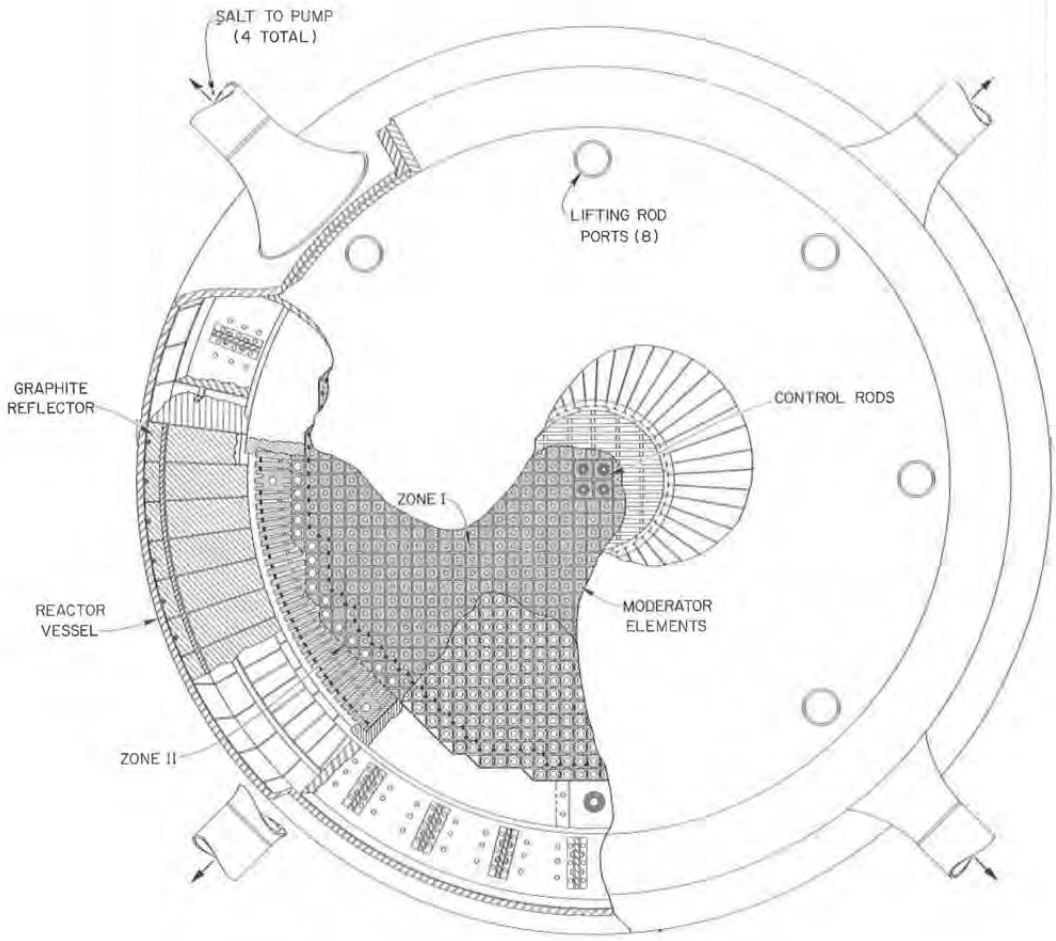
\includegraphics[width=\textwidth]{plan_view_vessel.png}
  \caption{Plan view of \gls{MSBR} vessel \cite{robertson_conceptual_1971}.}
  \vspace{-0.6em}
  \label{fig:ref_plan_msbr}
\end{figure}
\FloatBarrier

\begin{figure}[hbp!] % replace 't' with 'b' to 
  \centering
  \vspace{-0.3em}
  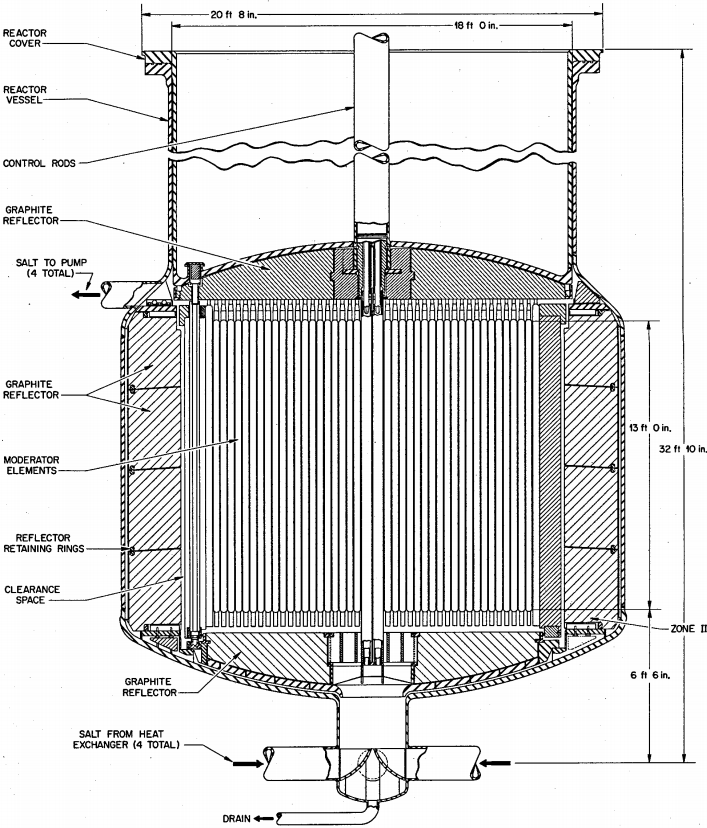
\includegraphics[width=\textwidth]{elev_view_vessel.png}
  \caption{Sectional elevation of \gls{MSBR} vessel \cite{robertson_conceptual_1971}.}
  \vspace{-0.6em}
  \label{fig:ref_sect_msbr}
\end{figure}
\FloatBarrier

There are eight graphite slabs with a width of 15.24 cm in zone II one to each other, one of which is illustrated in Fig.~\ref{fig:detail_plan_view}. The holes in the centers are for the core lifting rods used during the core replacement operations. These holes also allow a portion of the fuel salt to flow to the top of the vessel for cooling the top head and axial reflector. Fig.~\ref{fig:detail_plan_view} also demonstrates the 5.08-cm-wide annular space between the removable core graphite in zone II-B and the permanently mounted reflector graphite. This annulus, 100\% constists of fuel salt, provides space for moving the core assembly, helps compensate the out-of-roundness dimensions of the reactor vessel, and serves to reduce the damage flux at the surface of the graphite reflector blocks.

\begin{figure}[hbp!] % replace 't' with 'b' to 
  \centering
  \vspace{-0.3em}
  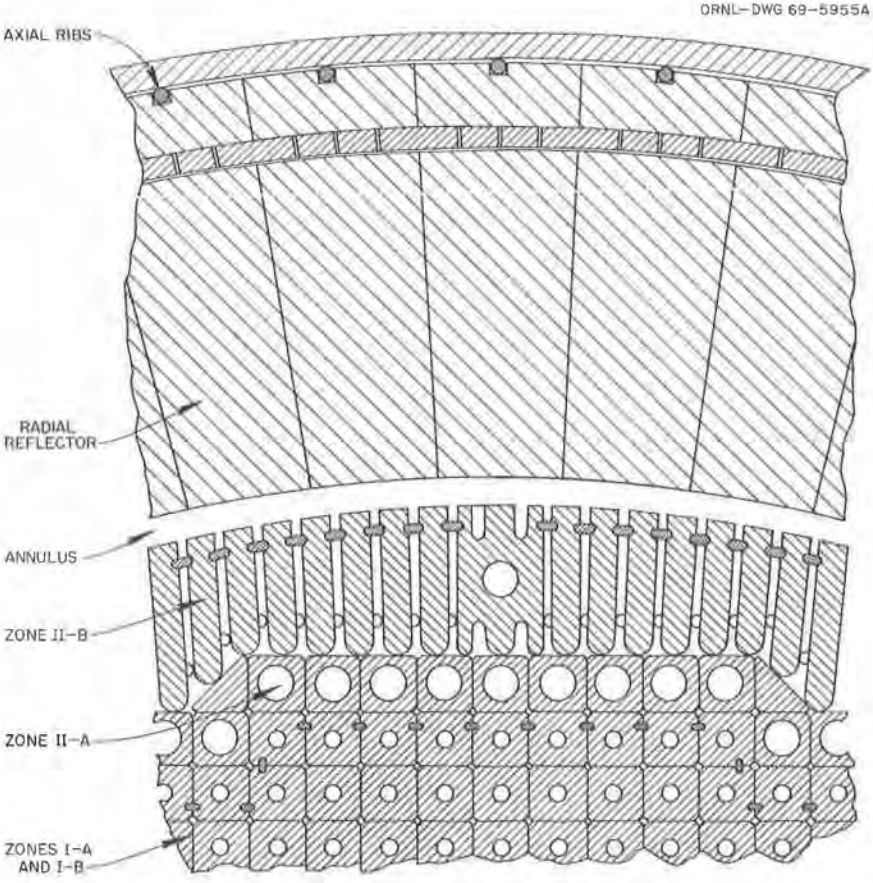
\includegraphics[width=\textwidth]{reflector_elements_ref.png}
  \caption{Detailed plan view of graphite reflector and moderator elements \cite{robertson_conceptual_1971}.}
  \vspace{-0.6em}
  \label{fig:detail_plan_view}
\end{figure}
\FloatBarrier

\subsection{Core zone I}
The central region of the core, called zone I, is made up of graphite elements, each $10.16$cm$\times$10.16cm$\times$396.24cm. In zone I, 13\% of the volume is fuel salt and 87\% is graphite. Zone I is composed of 1'320 graphite cells and 4 channels for control rods: two for graphite rods which both regulate and shim during normal operation, and two for backup safety rods to assure sufficient negative reactivity for emergency situations.

These graphite elements have a mostly rectangular shape with lengthwise ridges 
at each corner that leave space for salt flow elements. Various element sizes 
reduce the peak damage flux and power density in the center of the core prevent 
local graphite damage. Zone I is well-moderated which is necessarily to achieve desired fission power density. Figure~\ref{fig:I_element_ref} demonstrates the elevation and sectional views of graphite elements of zone I \cite{robertson_conceptual_1971} and these elements SERPENT model \cite{rykhlevskii_full-core_2017}.

\subsection{Core zone II}
The undermoderated zone, zone II, surrounds zone I. Combined with the bounding radial reflector, zone II serves to diminish neutron leakage. This zone is formed of two kinds of elements: elements like those in zone I with a larger channel diameter (zone II-A), and radial graphite slats (zone II-B). 

Zone II has 37\% salt by volume and each element has a fuel channel 
diameter of 6.604cm. It is divided into two different zones: zone II-A and zone 
II-B. The graphite elements for zone II-A are prismatic and have elliptical-shaped dowels running axially between the prisms and needed to isolate the fuel salt flow in zone I from that in zone II. Fig.~\ref{fig:II_element_ref} shows shape and dimensions of these graphite elements and SERPENT model. Zone II-B elements are rectangular slats spaced far enough apart to provide the 0.37 fuel salt volume fraction. The reactor zone II-B graphite 5.08cm-thick slats vary in the radial dimension (average width is 26.67cm) as shown in figure~\ref{fig:detail_plan_view}. Zone II serves as ``blanket" to achieve the best ``performance" associated with a high breeding ratio and a low fissile inventory. The neutron energy spectrum in zone II is made harder, to enhance the rate of thorium resonance capture relative to the fission rate, thus limiting the neutron flux in the outer core zone and reducing the neutron leakage \cite{robertson_conceptual_1971}. 

\begin{figure}[hbp!] % replace 't' with 'b' to 
  \centering
  \vspace{-0.3em}
  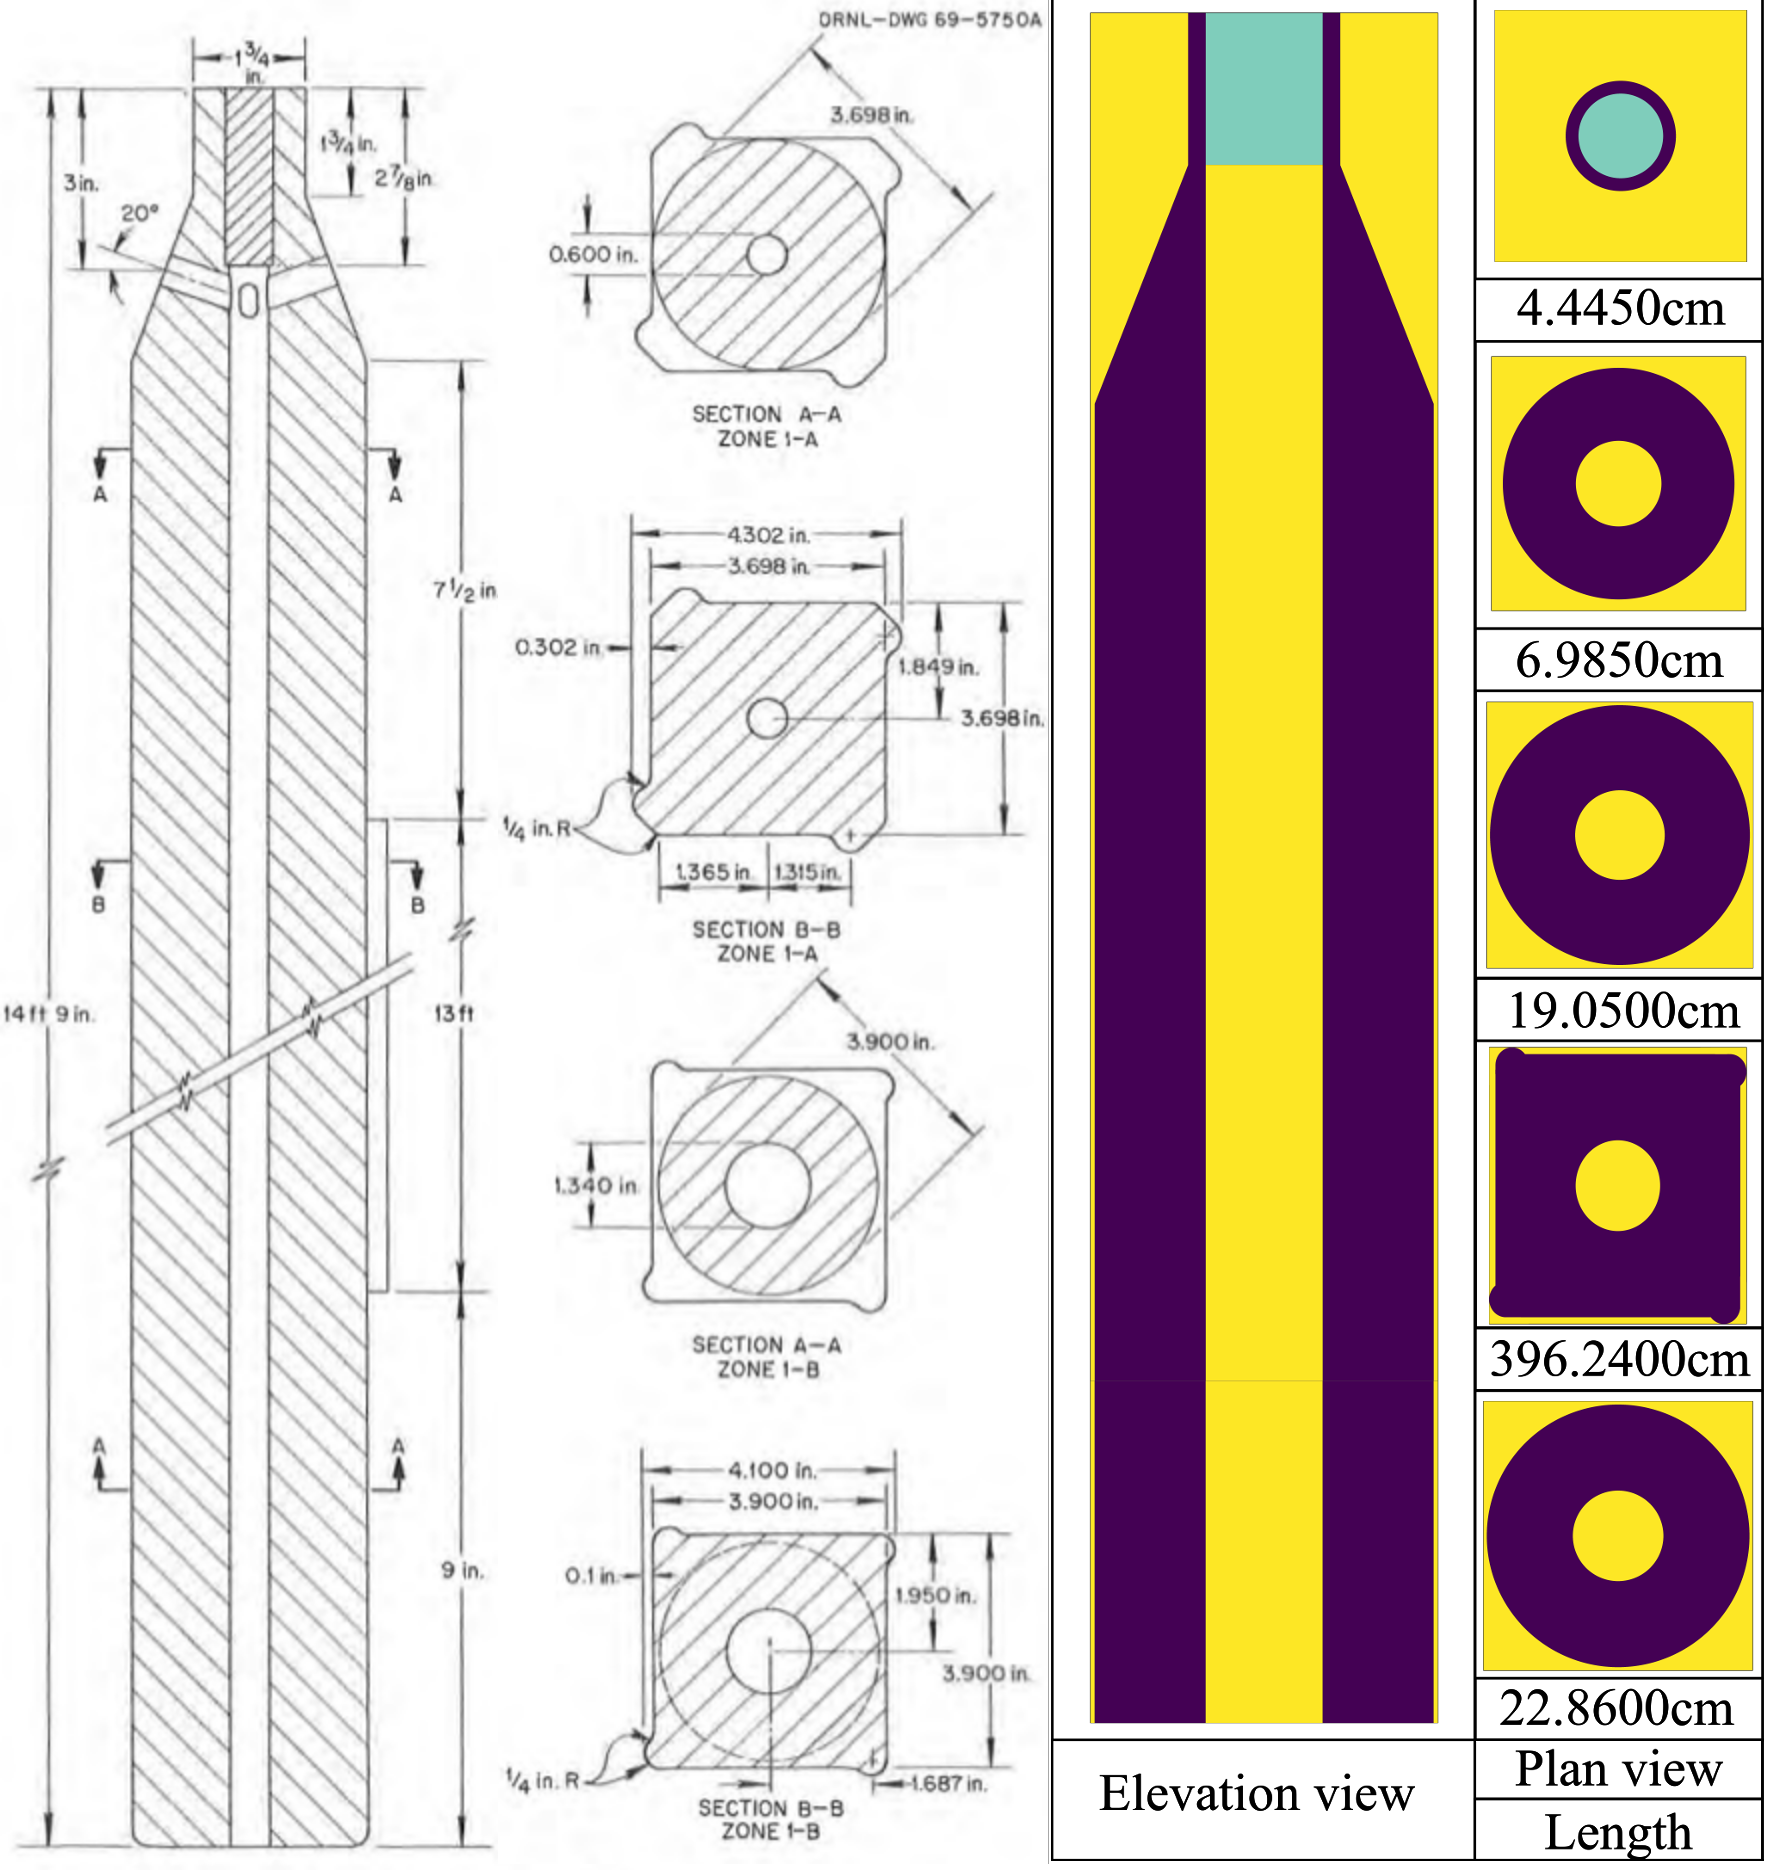
\includegraphics[width=\textwidth]{zone_I_element_ref.png}
  \caption{Graphite moderator elements for zone I \cite{robertson_conceptual_1971,rykhlevskii_full-core_2017}.}
  \vspace{-0.6em}
  \label{fig:I_element_ref}
\end{figure}
\FloatBarrier

\begin{figure}[hbp!] % replace 't' with 'b' to 
  \centering
  \vspace{-0.3em}
  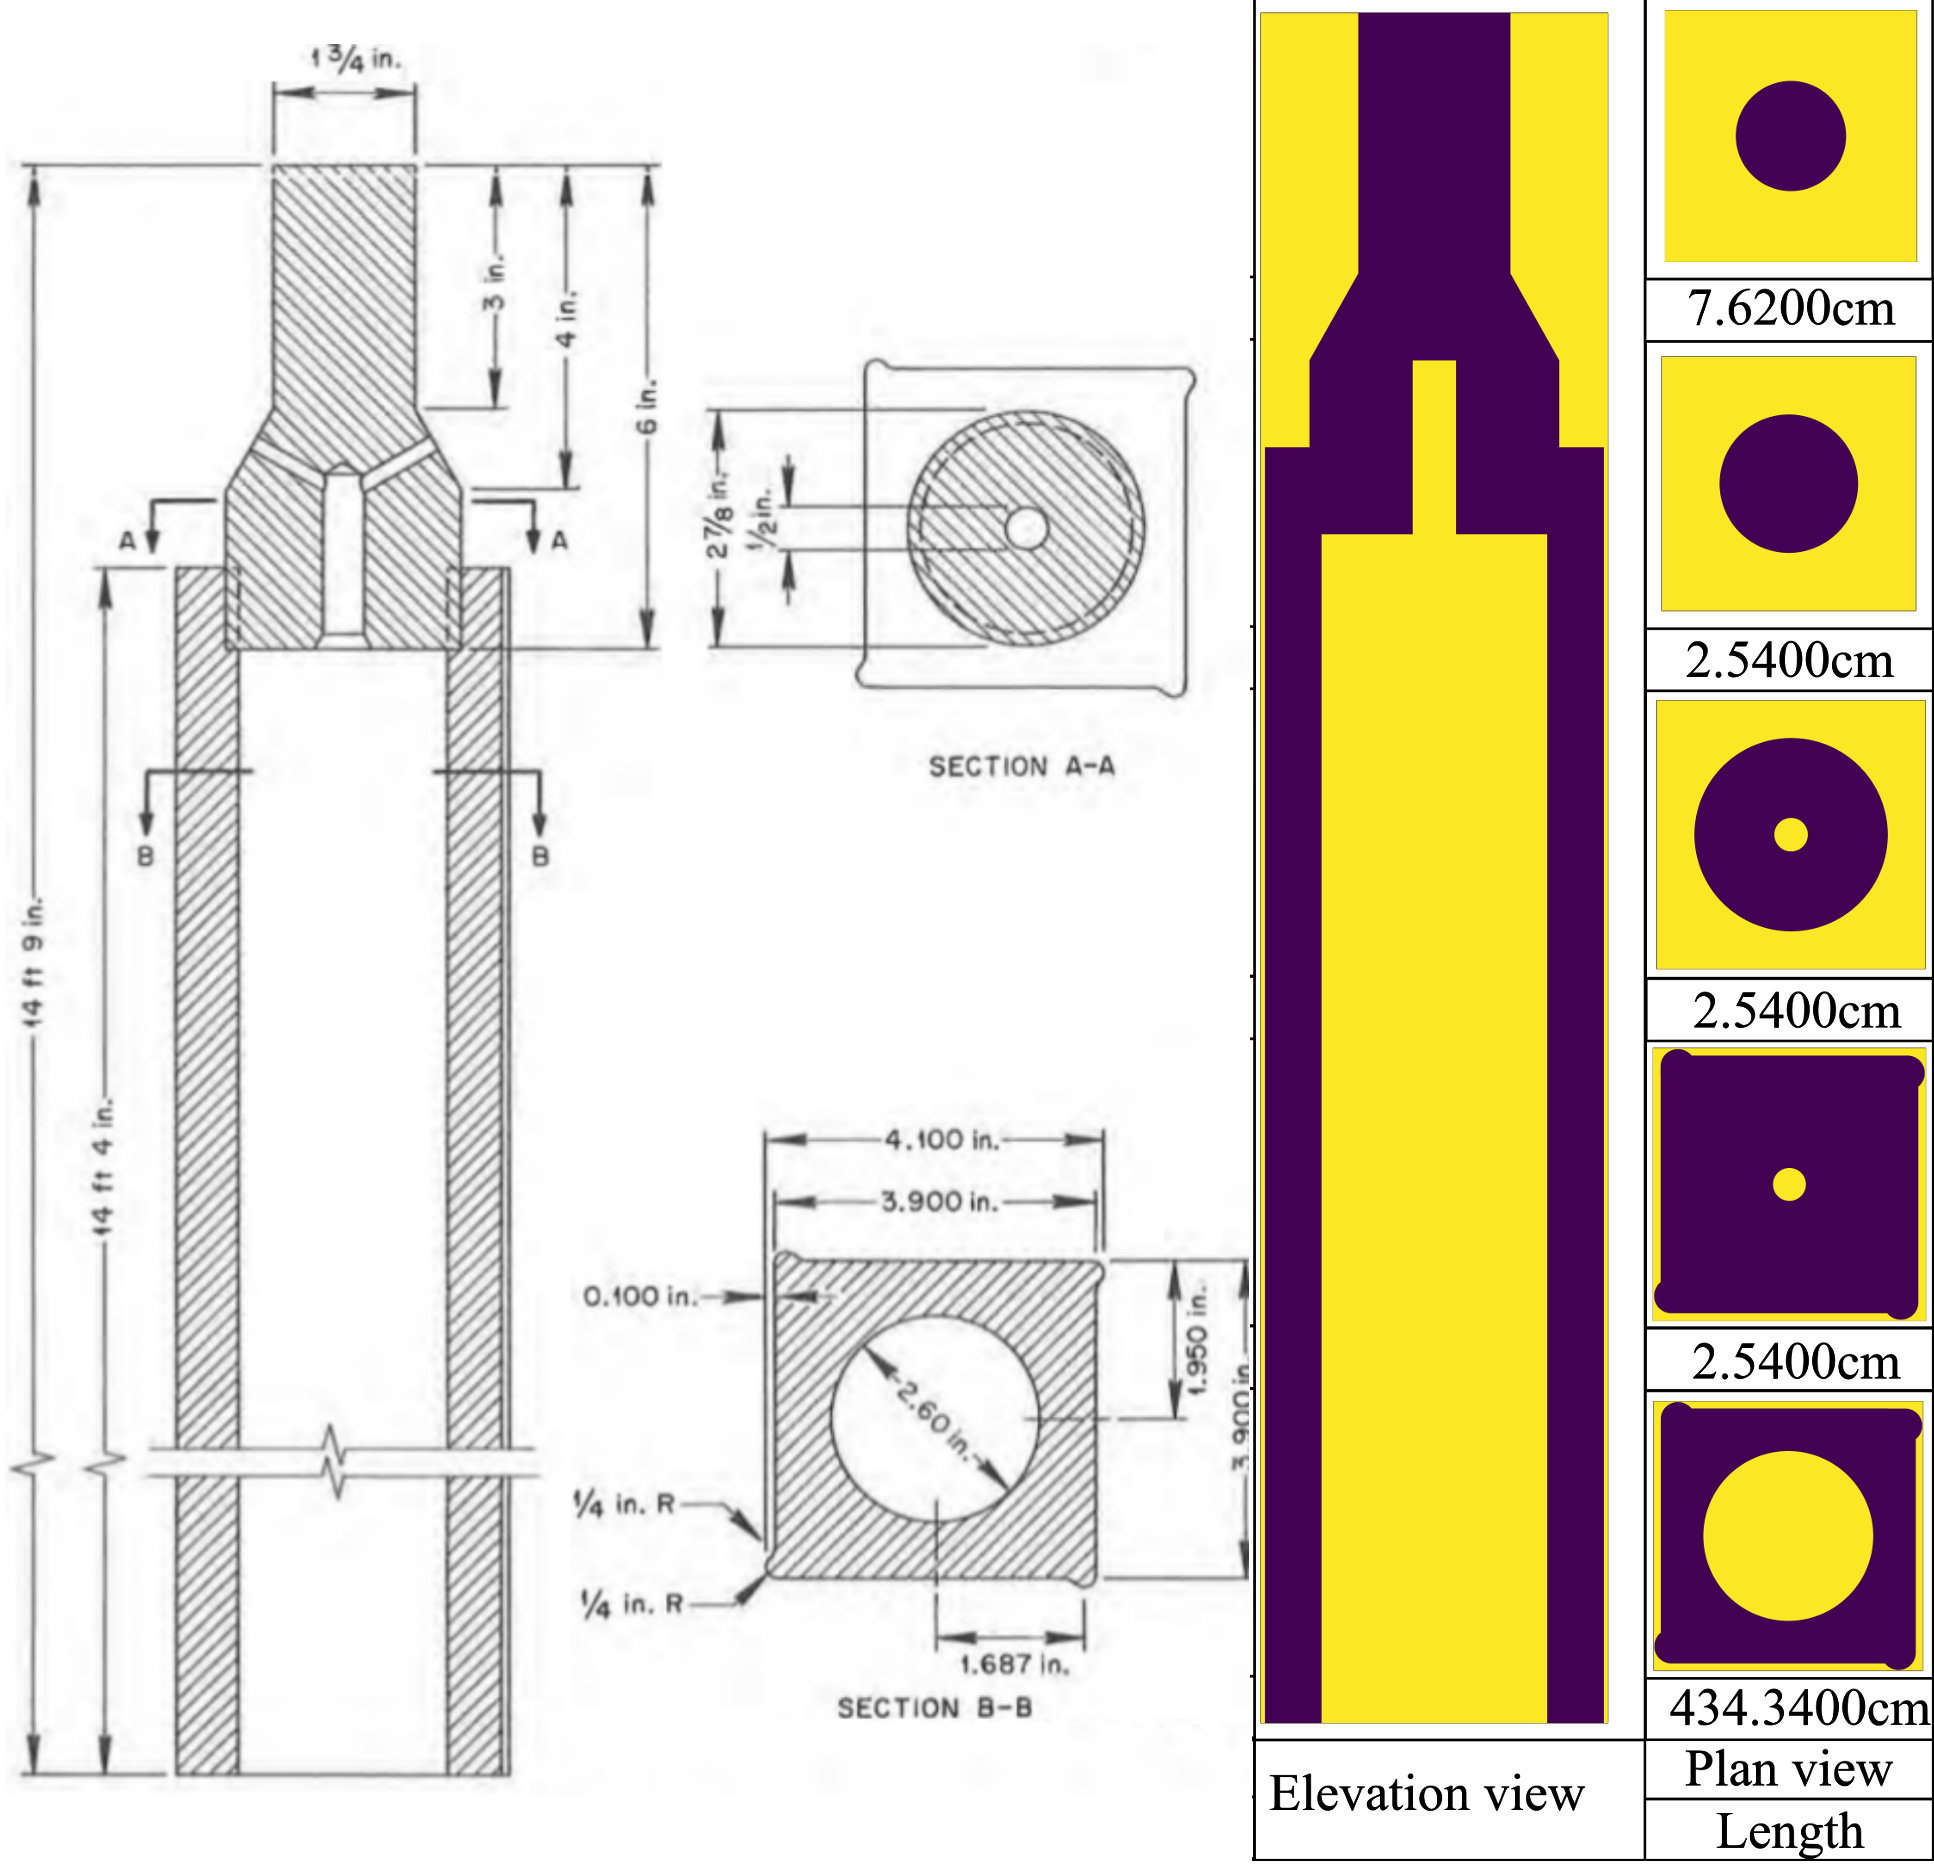
\includegraphics[width=\textwidth]{zone_II_element_ref.png}
  \caption{Graphite moderator elements for zone II-A \cite{robertson_conceptual_1971,rykhlevskii_full-core_2017}.}
  \vspace{-0.6em}
  \label{fig:II_element_ref}
\end{figure}
\FloatBarrier

\subsection{SERPENT 2 model}

To represent complex irregular \gls{MSBR} core geometry advanced geometry surfaces in SERPENT was employed. Fig.~\ref{fig:serpent_plan_view} shows the plan view of the whole-core configuration at the expected reactor operational level when both graphite control rods are fully inserted, and the safety rods are fully withdrawn. The safety rods only get inserted during an accident and was not considered in steady state simulation. 

Fig.~\ref{fig:serpent_sectional_view} shows the longitudinal section of the reactor. The violet color represents bare graphite, and the yellow represents fuel salt. The blue color shows Hastelloy-N, a material used for the plenum and vessel wall, and the white color is a void space. The model contains about 2000 geometry surfaces and 2066 calculation zones. In this thesis, all figures of the core were generated using the built-in SERPENT plotter.

\begin{figure}[hbp!] % replace 't' with 'b' to 
  \centering
  \vspace{-0.3em}
  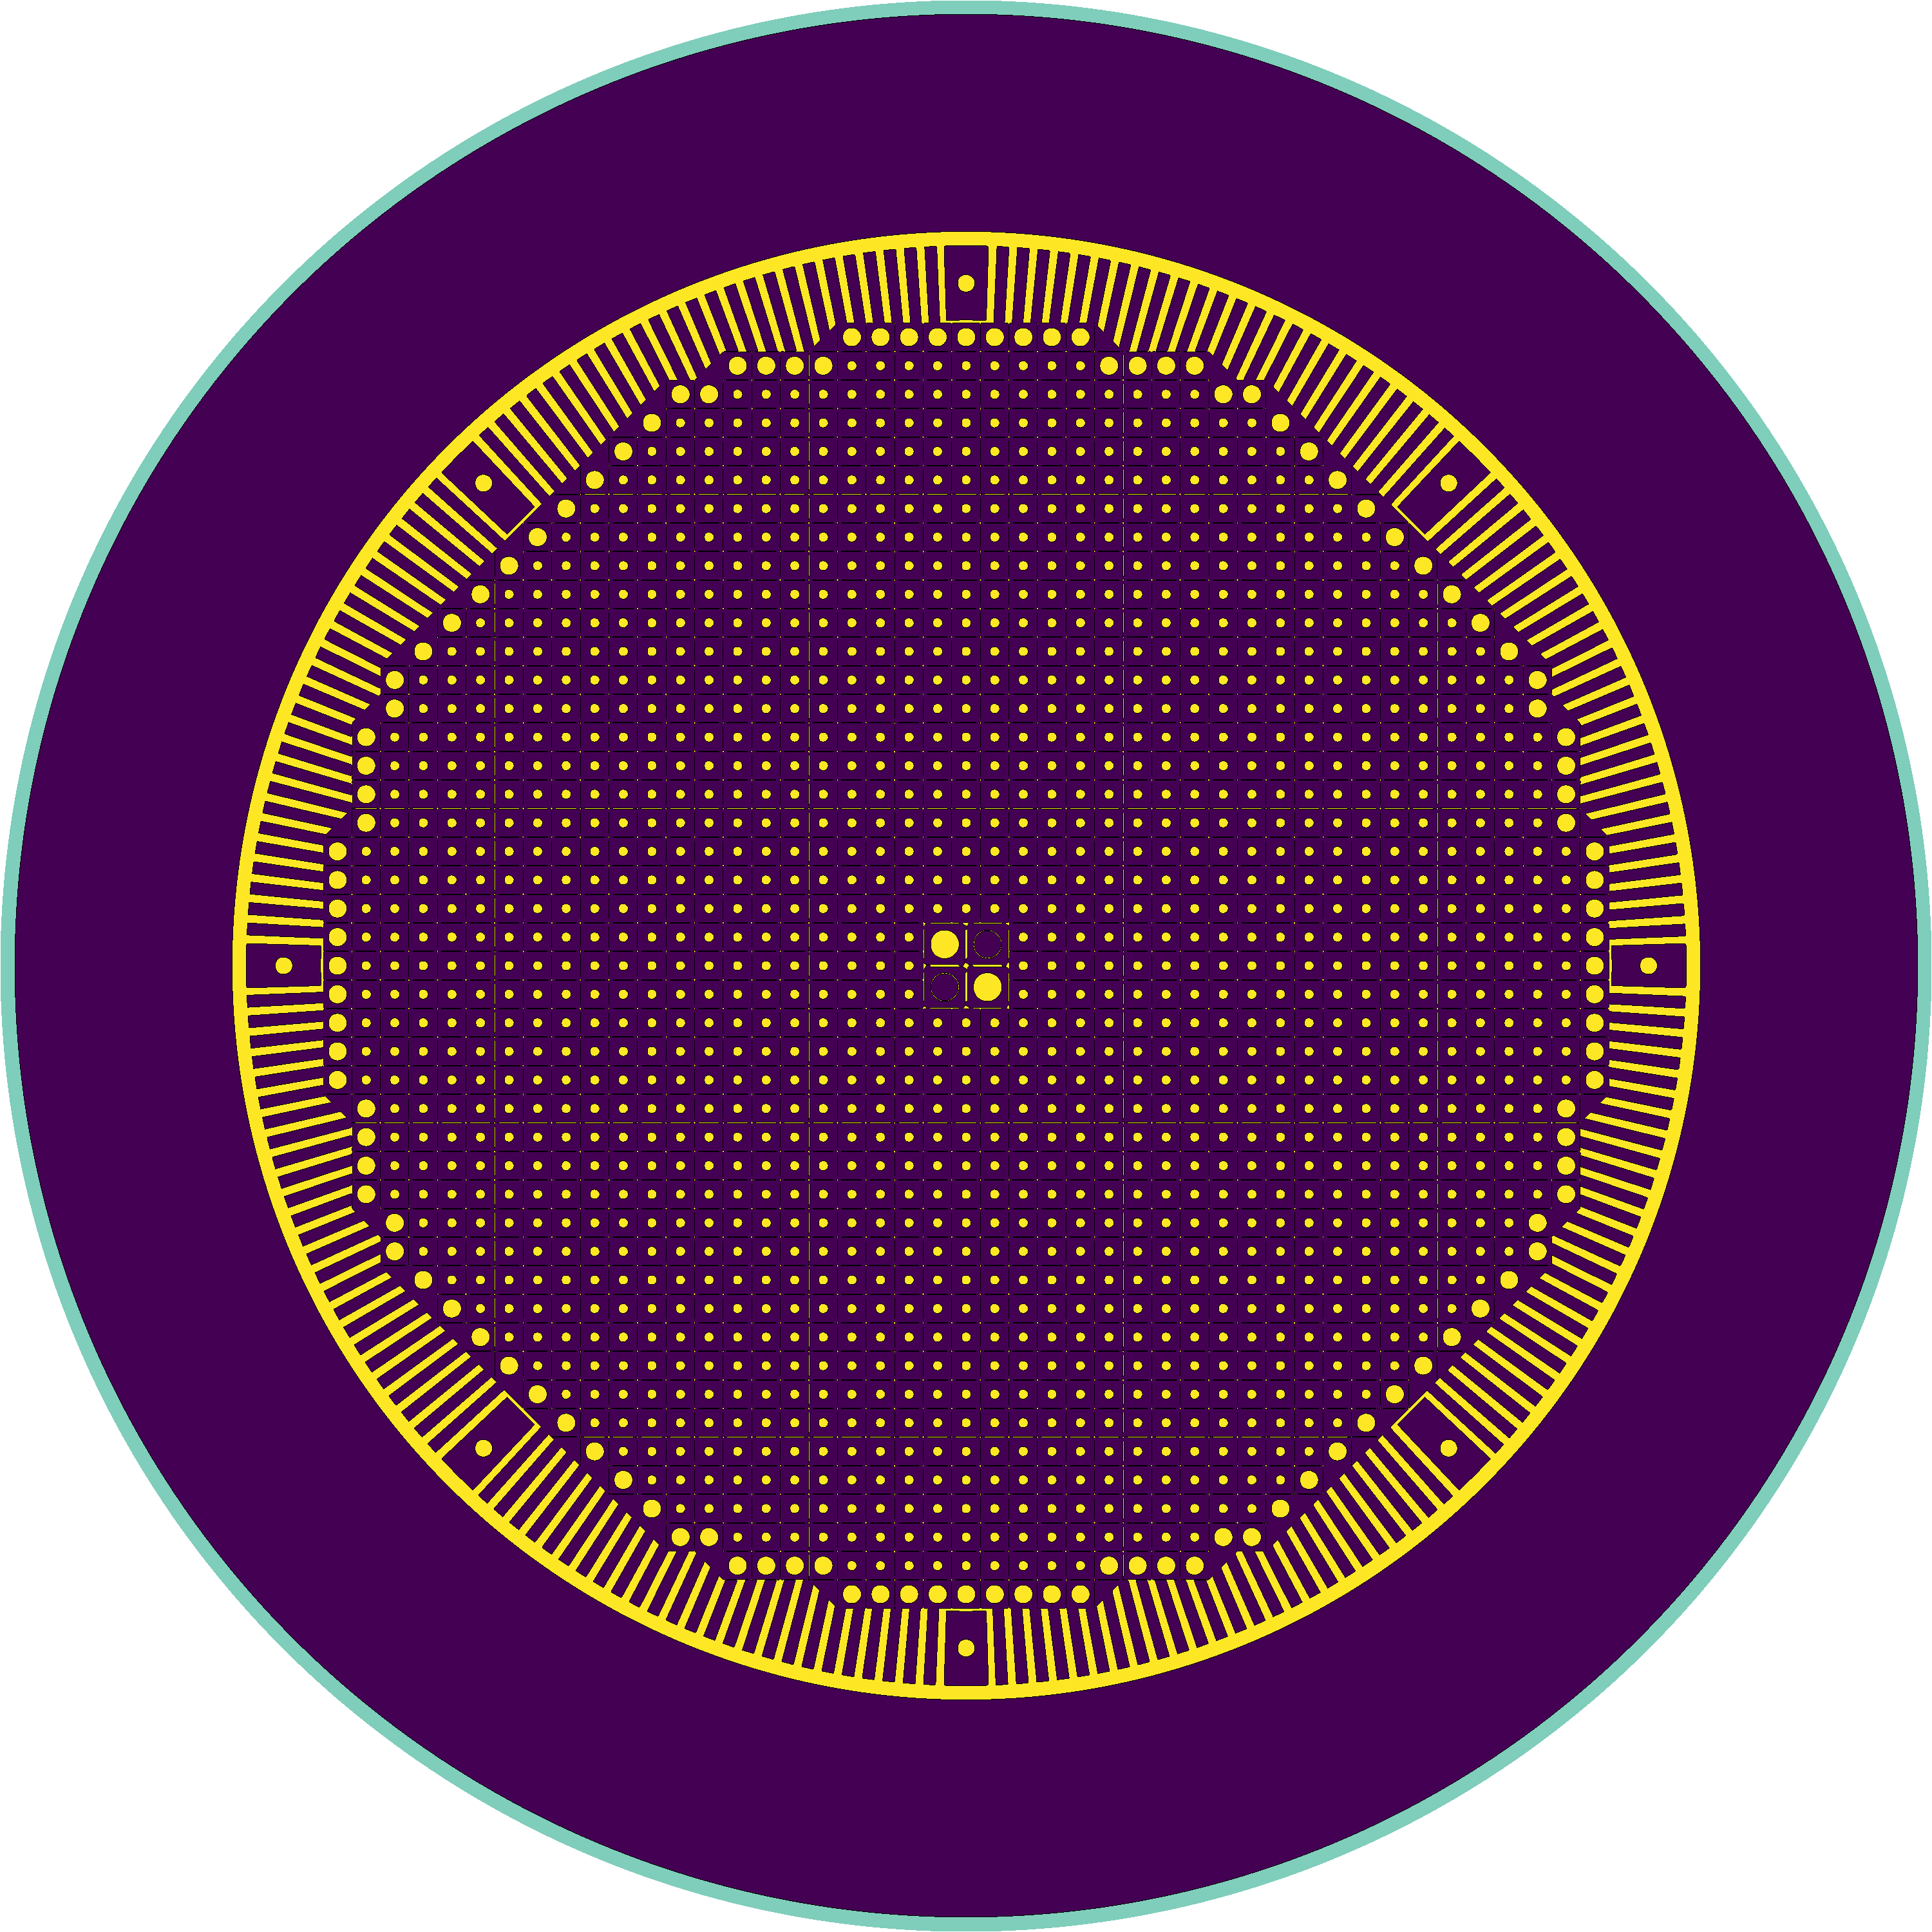
\includegraphics[width=1.05\textwidth]{plan_view_ser.png}
  \caption{Plan view of \gls{MSBR} model.}
  \vspace{-0.6em}
  \label{fig:serpent_plan_view}
\end{figure}
\FloatBarrier

\begin{figure}[hbp!] % replace 't' with 'b' to 
  \centering
  \vspace{-0.3em}
  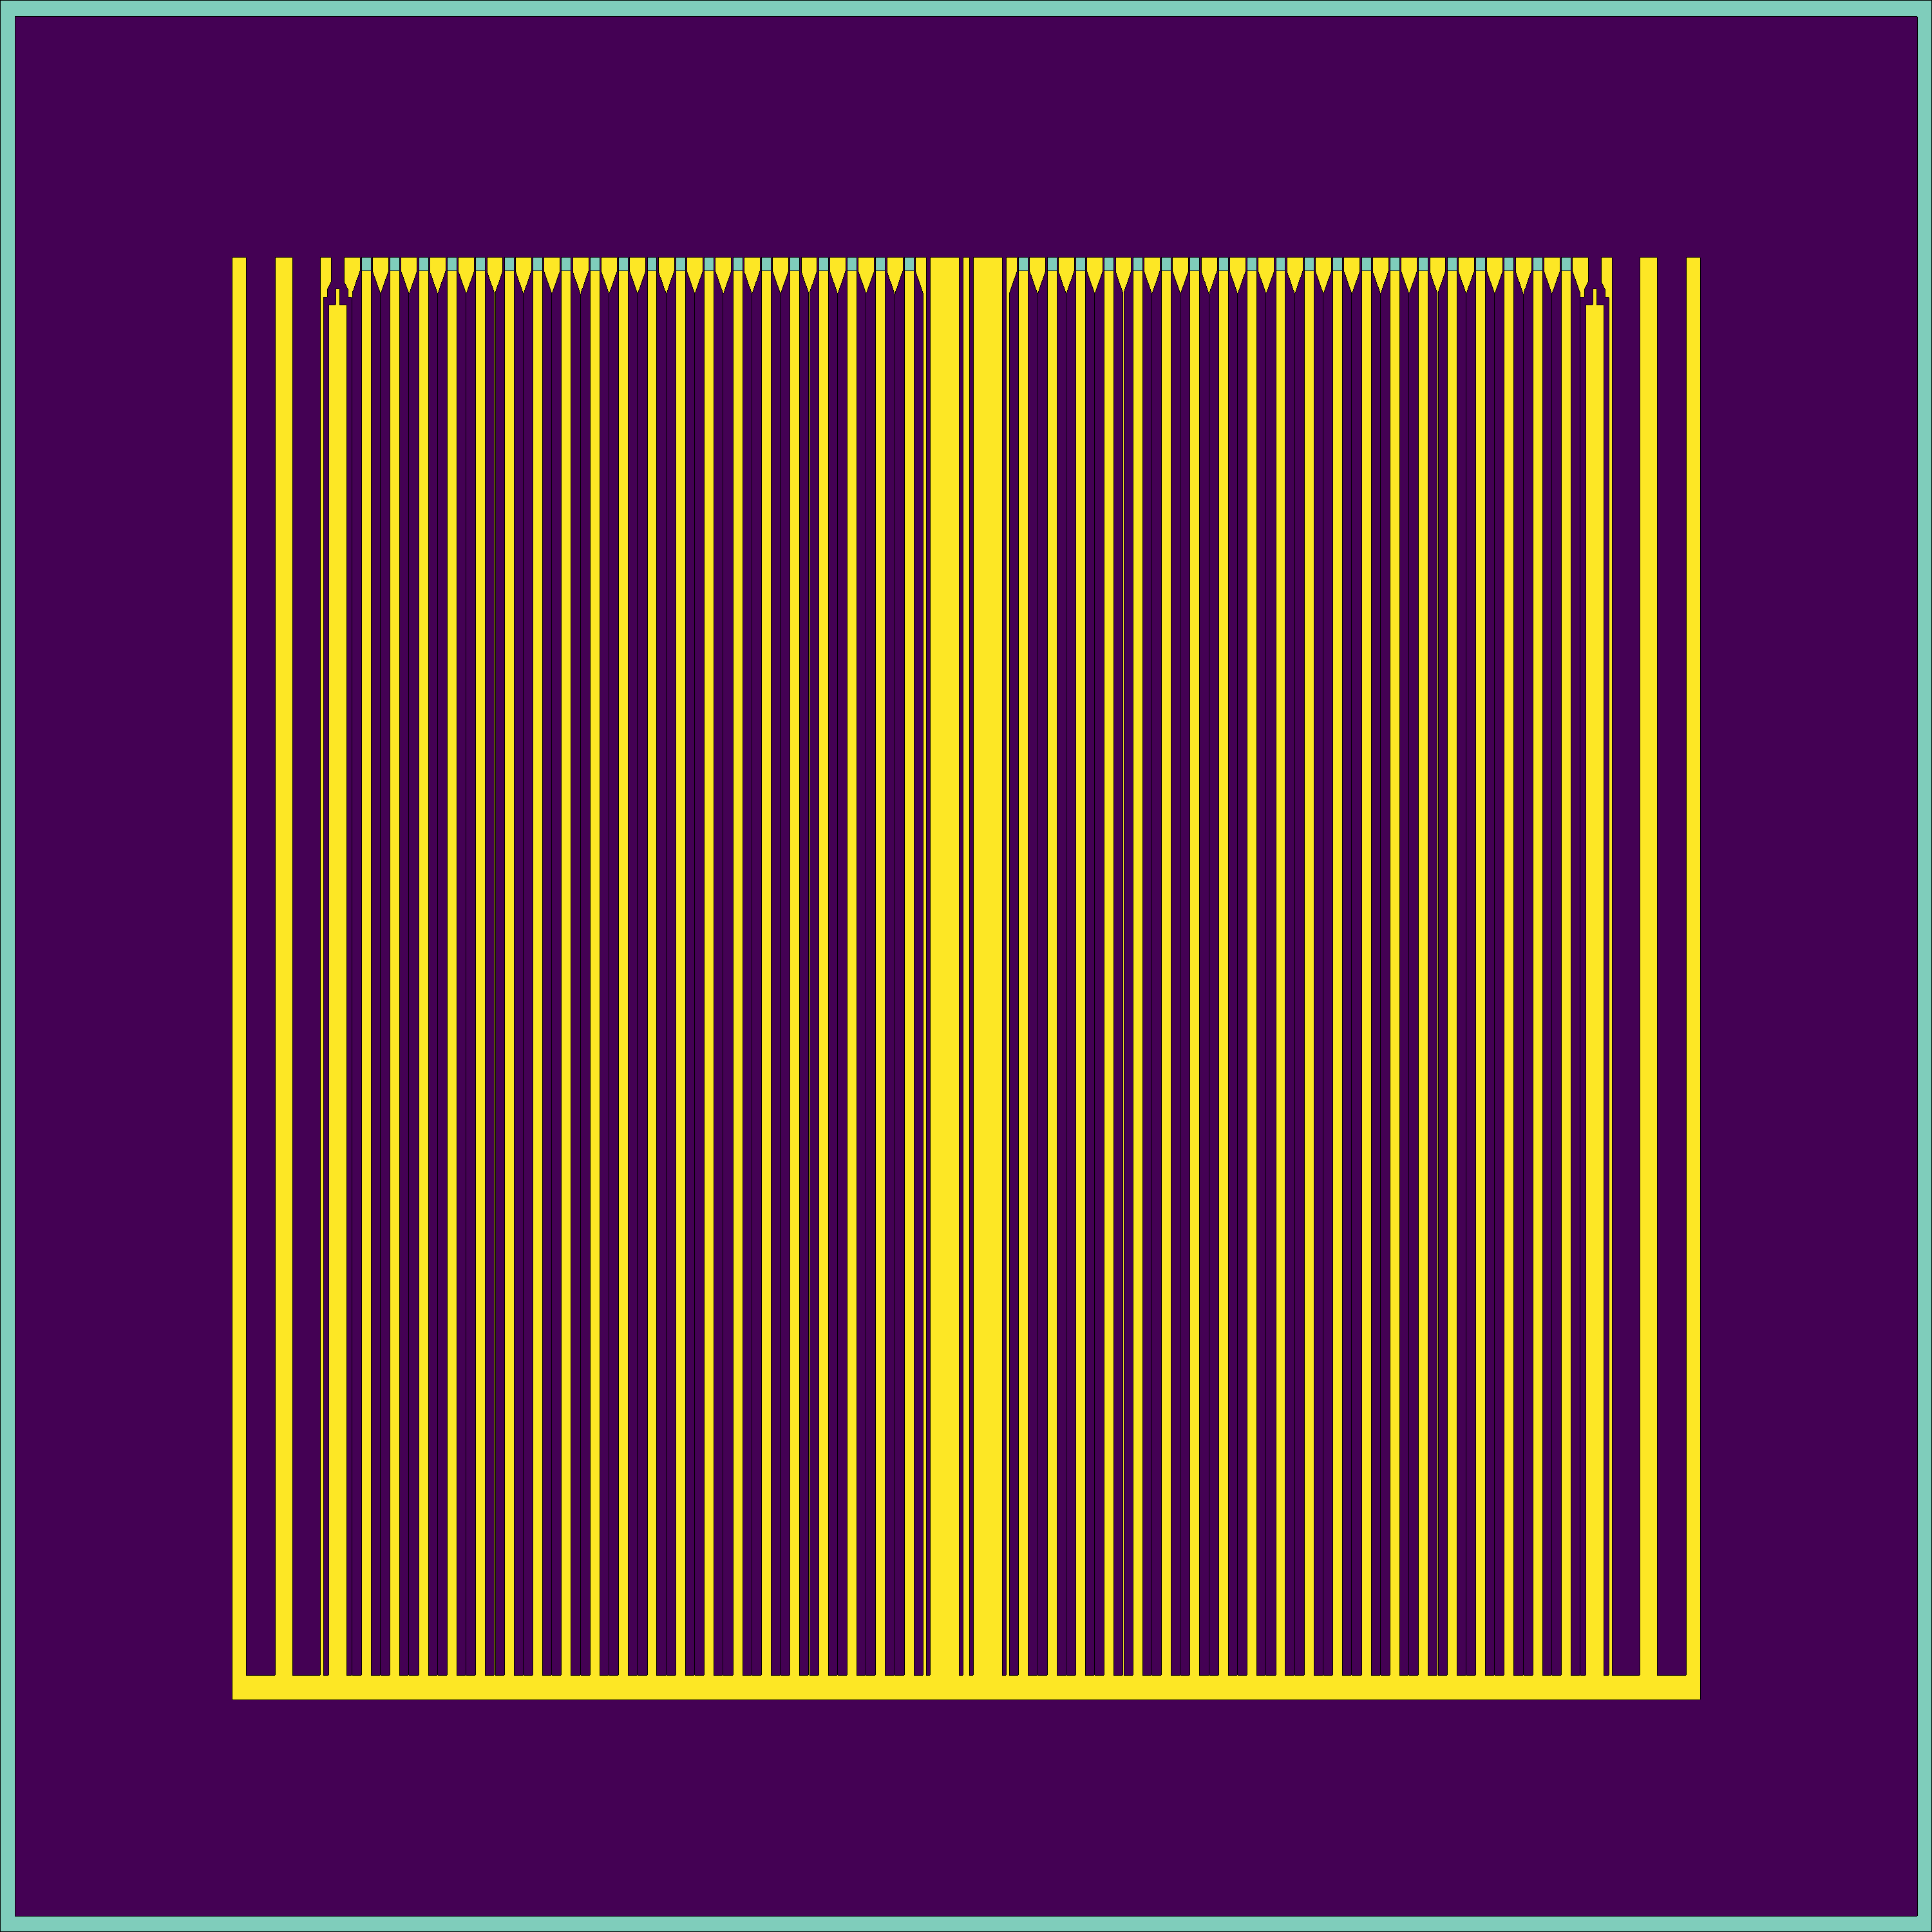
\includegraphics[width=1.05\textwidth]{sect_view_ser.png}
  \caption{Elevation view of \gls{MSBR} model.}
  \vspace{-0.6em}
  \label{fig:serpent_sectional_view}
\end{figure}
\FloatBarrier

In the model, zone I, zone II-A graphite blocks was described using circular cylinder and square cylinder surface types, lengthwise ridges at each corner mentioned earlier was specified using dodecagonal cylinder surfaces and general planes. Zone I of the core was described using square lattice inscribed in the octagonal cylinder surfaces to accurately represent geometry of that region.

The main challenge was accurately represent zone II-B because it has irregular elements with sophisticated shape. From the ORNL report \cite{robertson_conceptual_1971}, the suggested design of zone II-B has 8 irregularly-shaped graphite elements every 45$^\circ$ as well as salt channels (figure~\ref{fig:detail_plan_view}). These graphite elements were simplified into right-circular cylindrical shapes  with central channels. Fig.~\ref{fig:serpent_zoneII} illustrates this core region in SERPENT model. Volume of fuel salt in zone II kept exactly 37\%, consequently, this simplification did not considerably change neutronics of the core. This is the only simplification made to the \gls{MSBR} conceptual geometry in this work. 

\begin{figure}[hbp!] % replace 't' with 'b' to 
  \centering
  \vspace{-0.3em}
  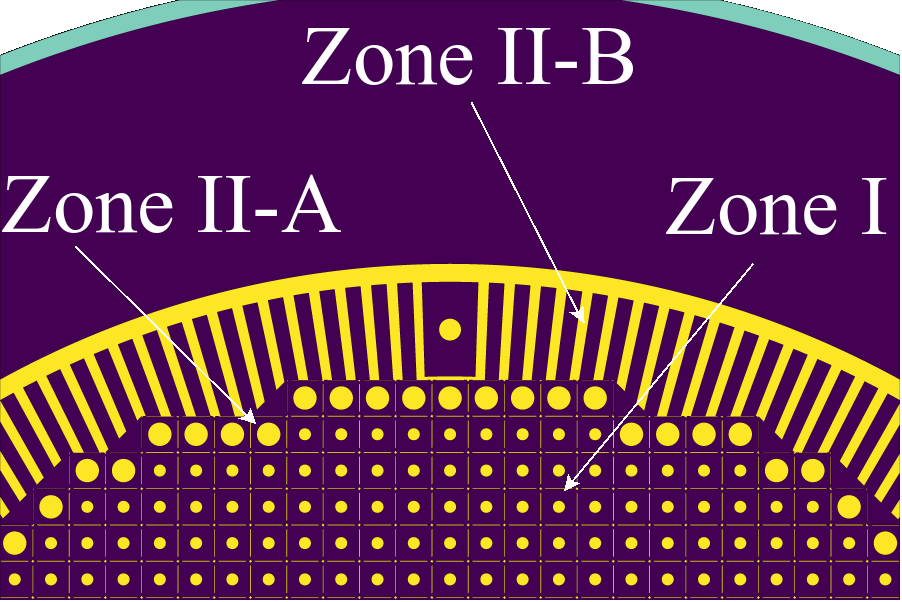
\includegraphics[width=1.05\textwidth]{ser_zone_II.png}
  \caption{Detailed view of \gls{MSBR} zone II model.}
  \vspace{-0.6em}
  \label{fig:serpent_zoneII}
\end{figure}
\FloatBarrier

\subsection{Material composition and normalization parameters}
The fuel salt, the reactor graphite, and the modified Hastelloy-N are materials 
unique of the \gls{MSBR} and were created at \gls{ORNL}. The initial fuel salt used the same density (3.35g/cm$^3$) and composition LiF-BeF$_2$-ThF$_4$-$^{233}$UF$_4$ (71.8-16-12-0.2 mole \%) as the \gls{MSBR} design \cite{robertson_conceptual_1971}. The lithium in the molten salt fuel is a fully enriched $^{7}$Li because 
$^{6}$Li is a very strong neutron poison and becomes tritium upon neutron 
capture. A power level of 2250 MW$_{th}$, thermal efficiency of 44.4\% (yielding net electrical output 1000 MW$_e$), total fuel salt volume of 48.7 m$^3$, and fissile mass in salt 1303.7 kg were all taken from ORNL report \cite{robertson_conceptual_1971}.

For cross section generation, JEFF-3.2 was employed 
\cite{oecd/nea_data_bank_jeff-3.2_2014}. The specific temperature was fixed for each 
material to correctly model the Doppler-broadening of resonance peaks when 
Serpent generate problem-oriented nuclear data library. The isotope composition of each material at the initial state was described in detail in the MSBR conceptual design study \cite{robertson_conceptual_1971} and has been applied to Serpent model without any modification. 

\section{Results}
This section presents calculation results, such as the effective multiplication 
factor for whole core, neutron flux spectrum, temperature reactivity 
coefficients, and compares the results against those obtained by Park \emph{et al.} using Monte Carlo \gls{MCNP}6 \cite{park_whole_2015}. 

Figure~\ref{fig:park_detailed_view} illustrates Park \emph{et al.} model which ignores lengthwise graphite ridges at each corner of each graphite element in zone I, II-A, and significantly simplifies in zone II-B and annulus. The normalized neutron flux distribution is calculated for the whole core using continuous-energy nuclear data. The temperature coefficients for both fuel salt solution and reactor graphite are computed by comparing effective multiplication factors for two temperatures in the working range.

\begin{figure}[htp!] % replace 't' with 'b' to 
  \centering
  \vspace{-0.3em}
  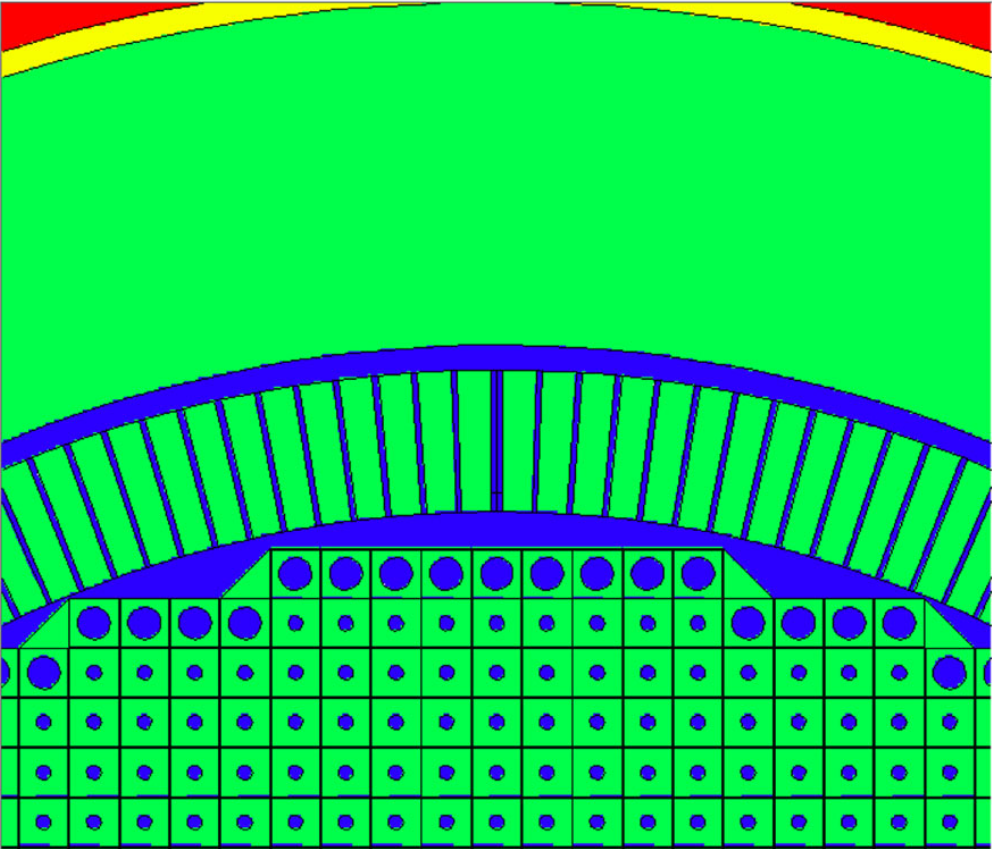
\includegraphics[width=0.9\textwidth]{park_detailed_view.png}
  \caption{Detailed plan view of Park (MCNP6) model \cite{park_whole_2015}.}
  \vspace{-0.6em}
  \label{fig:park_detailed_view}
\end{figure}
 	
\subsection{Neutron spectrum}
Fig.~\ref{fig:spectrum} demonstrates the normalized neutron flux spectrum for 
the whole core in the energy range from $10^{-9}$ to $10$ MeV. The results show 
close fit with the MCNP simulation \cite{park_whole_2015}, especially in 
thermal energy range.  
\begin{figure}[t!] % replace 't' with 'b' to force it to 
  \centering
  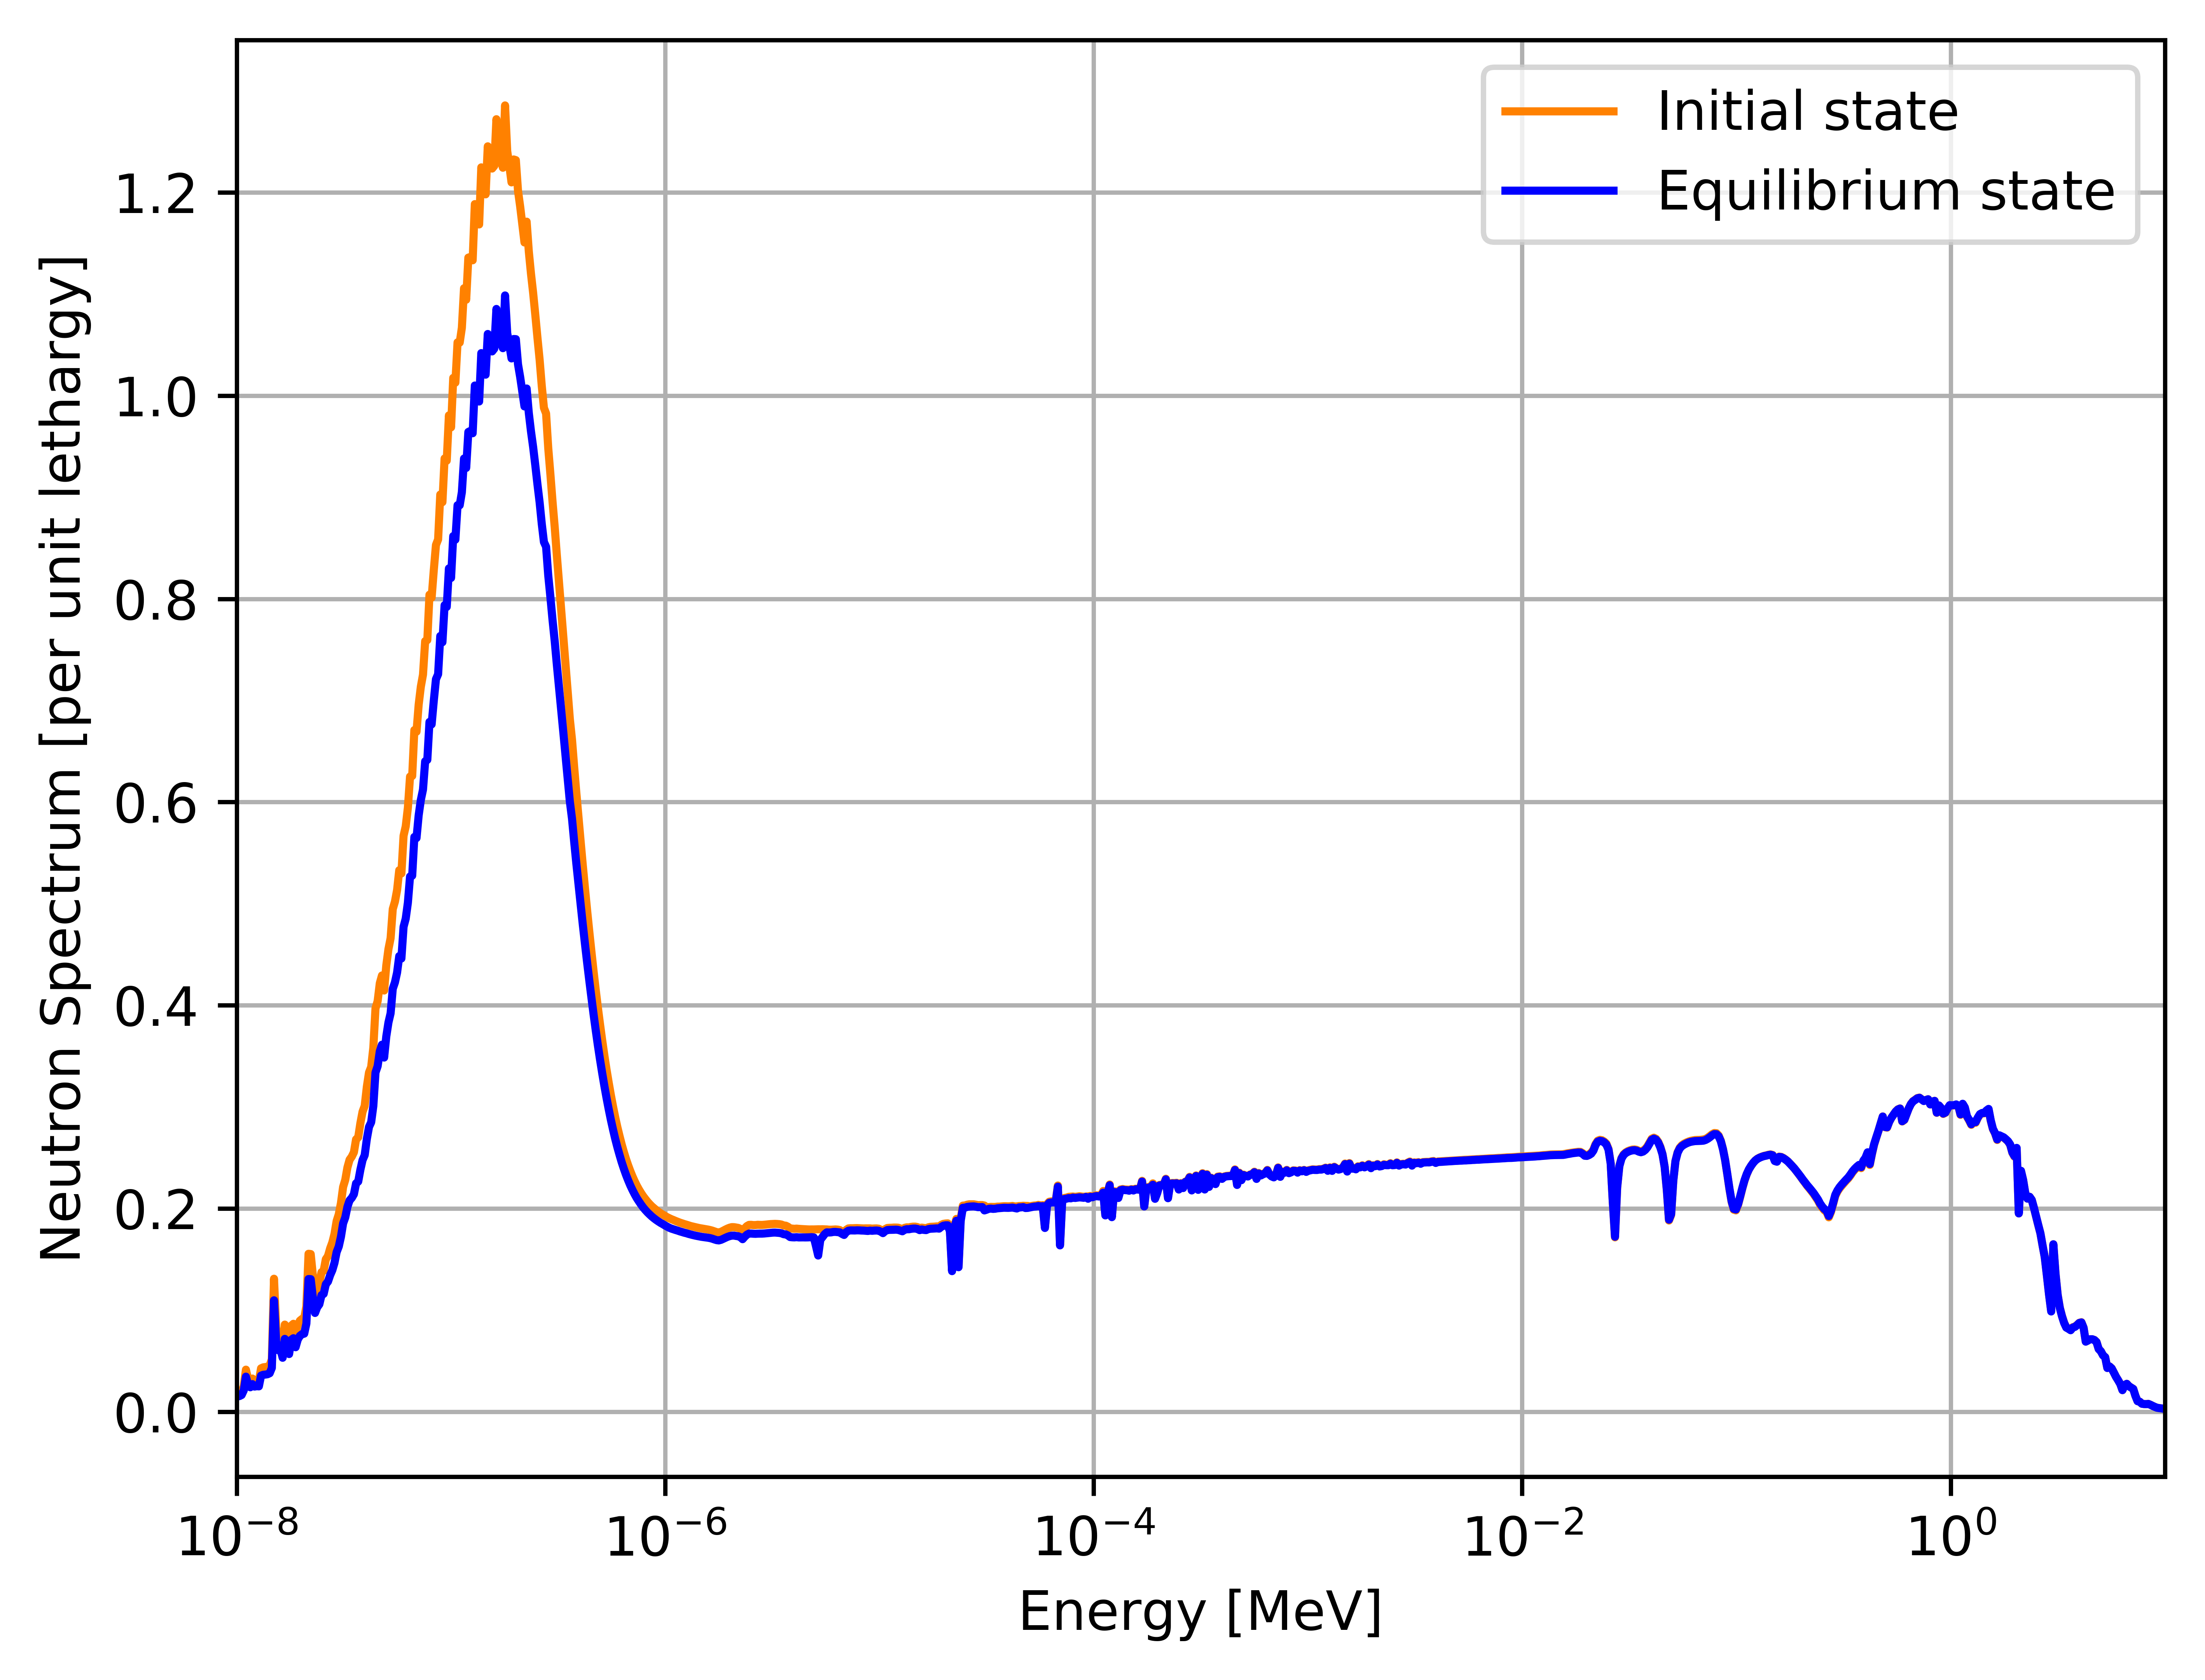
\includegraphics[width=1.05\linewidth]{spectrum.png} \caption{Neutron flux 
  spectrum of \gls{MSBR} for MCNP6 and SERPENT model.}
  \label{fig:spectrum}
\end{figure}
It is important to obtain the epithermal and thermal spectrum to produce 
$^{233}$U from $^{232}$Th because radiative capture cross section of thorium 
monotonically decreases from $10^{-10}$ MeV to $10^{-5}$ MeV. Hardening the 
spectrum tends to significantly increase resonance absorption in thorium and 
decrease the absorptions in fissile and construction materials. Thus, a 
signficant amount fissile material will be needed to make the reactor critical.

\subsection{Effective multiplication factor}
Table~\ref{tab:keff} shows the effective multiplication factor for both MCNP6 
and Serpent 2 whole core models. The factor obtained using Serpent 2 is 300 pcm 
lower than that obtained by Park \emph{et al.} using MCNP6 
\cite{park_whole_2015}. Standard deviations are 5 and 9 pcm, respectively. The 
discrepancy is likely due to simplificiations to the Zone II geometry model 
used in Park \emph{et al.}
%%%%%%%%%%%%%%%%%%%%%%%%%%%%%%%%%%%%%%%%
\captionsetup[table]{
  labelsep = newline,
  name = TABLE, justification=justified,
  singlelinecheck=false,%%%%%%% a single line is centered by default
  labelsep=colon,%%%%%%
  skip = \medskipamount}
\begin{table}[h!]
%\centering
\caption{Effective multiplication factor of whole core model.}
\begin{tabular}{p{0.15\linewidth} p{0.3\linewidth} p{0.3\linewidth}} \toprule
      & Serpent2      & MCNP6 \cite{park_whole_2015}          \\ \midrule
K$_{eff}$  & 1.00389$\pm$0.00005 & 1.00736$\pm$0.00009
\\
\bottomrule
\end{tabular}
  \label{tab:keff}
\end{table}
%%%%%%%%%%%%%%%%%%%%%%%%%%%%%%%%%%%%%%%%%%%%%%%%%%%%%%%%%%%%%%%%%%%%%%%%%%%%%%%%
\subsection{Temperature effect of reactivity}
Table~\ref{tab:tcoef} shows temperature effects on reactivity calculated in 
this work as compared to both \cite{park_whole_2015} and 
\cite{robertson_conceptual_1971}. Uncertainty for each temperature coefficient 
also appears in Table~\ref{tab:tcoef}. The main physical principle underlying 
the reactor temperature feedback is an expansion of matter when it is heated.  
When the fuel salt temperature increases, the density of the salt decreases, 
but at the same time, the total volume of fuel salt in the core remains 
constant because it is bounded by the graphite. When the reactor graphite 
temperature grows, the density of graphite declines creating additional space 
for fuel salt. To determine temperature coefficients, the cross-section 
temperatures for fuel and moderator were changed from 900K to 1200K. Three 
different cases were considered:
\begin{enumerate}  \item Temperature of fuel salt rising from 900K to 1200K.
\item Temperature of graphite rising from 900K to 1200K.  \item Whole reactor 
        temperature rising from 900K to 1200K.
\end{enumerate}

%%%%%%%%%%%%%%%%%%%%%%%%%%%%%%%%%%%%%%%%
\captionsetup[table]{
  labelsep = newline,
  name = TABLE, justification=justified,
  singlelinecheck=false,%%%%%%% a single line is centered by default
  labelsep=colon,%%%%%%
  skip = \medskipamount}
\begin{table}[h!]
%\centering
  \caption{Temperature coefficients of reactivity.}
\begin{tabular}{p{0.22\linewidth} p{0.22\linewidth} p{0.21\linewidth} 
        p{0.15\linewidth}} \toprule
   Reactivity coefficient [pcm/K]  & Serpent2      & MCNP6 
        \cite{park_whole_2015}   & Reference \cite{robertson_conceptual_1971}      
        \\ \midrule
Fuel salt        & $-3.70\pm0.016$ & $-3.20\pm0.05$ & $-3.22$ \\ \midrule
Moderator        & $+2.33\pm0.027$ & $-0.11\pm0.05$ & $+2.35$ \\ \midrule
Total            & $-1.57\pm0.033$ & $-3.21\pm0.04$ & $-0.87$ \\
\bottomrule
\end{tabular}
  \label{tab:tcoef}
\end{table}
%%%%%%%%%%%%%%%%%%%%%%%%%%%%%%%%%%%%%%%%%%%%%%%%%%%%%%%%%%%%%%%%%%%%%%%%%%%%%%%%
In the first case, changes in the fuel temperature only impact fuel density. In 
this case, the geometry is unchanged because fuel is a liquid. However, when 
the moderator heats up, both the density and the geometry change due to thermal 
expansion of the solid graphite blocks and reflector. Accordingly, the new 
graphite density was calculated using a linear temperature expansion 
coefficient of 1.3$\times10^{-6}$1/K \cite{robertson_conceptual_1971}. A new 
geometry input was created based on this information.

The fuel temperature coefficient (FTC) is negative due to thermal Doppler 
broadening of the resonance capture cross sections in the thorium and is in a 
good agreement with early research 
\cite{robertson_conceptual_1971,park_whole_2015}. The moderator temperature 
coefficient is positive due to changing density and would increase during 
reactor operation because of spectrum hardening along with fuel depletion 
\cite{park_whole_2015}. Finally, the total temperature coefficient of 
reactivity is relatively large and negative, despite graphite components, and 
affords excellent reactor stability and controllability.